\section{Orbit Architecture}
\label{blDOOrb}
In this section the design options in the orbit architecture tree as seen in Figure-ref(???) to Figure-ref(???) are described. The orbits are divided in four categories: \ac{LEO}, \ac{MEO}, \ac{GEO} and finally \ac{HEO}. Certain orbits like transfer orbits and hyperbolic and parabolic trajectories are not included as they are not relevant for the mission.

After the main categories there are subdivisions, which can in turn have subdivisions as well. These subdivisions list the special orbits types that are possible, sometimes there is also a block called ``other''. This is because special orbit types have special constraints, as will be detailed in later sections; whereas the ``other'' block is there to represent all the other possible orbits.

All orbits are assumed to be Keplerian orbits, as such the orbit is a plane located in 3D space. Therefore six elements will define the position of the satellite. One example of these elements are the classical orbital elements. The elements are the semimajor axis $a$, the eccentricity $e$, the inclination $i$, the right ascension of the ascending node \Omega, the argument of perigee \omega and finally the true anomaly \nu. As a reference for the last four terms Figure-\ref{OrbElements} may be used.
\begin{figure} [H]
	\begin{center}
         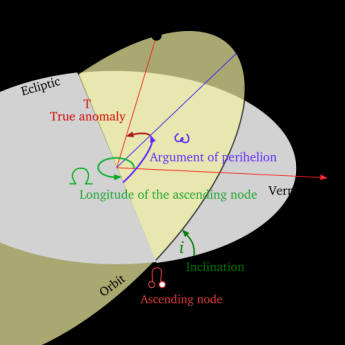
\includegraphics[width=1.0\textwidth,angle=0]{chapters/img/OrbElements.png}
	\caption{Definitions of the inclination $i$, the right ascension of the ascending node \Omega, the argument of perigee \omega and the true anomaly \nu.}
	\label{OrbElements}
	\end{center}
	\end{figure}
The most important of the four Keplerian elements during this part of the design are the semimajor axis, the eccentricity and the inclination. The remaining elements are not considered until detailed design.

The following sections will each describe one of the four main categories. They are described in the order listed in the first paragraph of this section. However, first the most common orbits are discussed in the following paragraphs.

\subsection {Common orbits}
\label{blOrbCommon}
Some special orbits are repeated multiple times in the orbit architecture trees as shown in Figure-ref(???) to Figure-ref(???). These common orbits are the polar orbit, the sun synchronous orbit, the sun synchronous polar orbit, the frozen orbit and the repeat orbit.

\begin{enumerate}
	\item Polar orbit:
	This orbit is unique in that the satellite will pass over or close to both poles during a single revolution. As such the angle of incidence $i$ is close to  \pm 90 [deg]. This setup allows for near global coverage.
	\item Sun synchronous orbit:
	An orbit where the satellite passes over the same ground area at the same local time each revolution. At increasing altitude the inclination increases as well, so above approximately 5000 [km]\cite{larson} this orbit tends to lose its usefulness. 
	\item Sun Synchronous Polar orbit:
	A combination of the previous two items, for this orbit to keep the same local time the altitude should be as low as possible.
	\item Frozen orbit:
	An orbit where there are no long-term changes in argument of perigee and eccentricity. The eccentricity is determined based on a given semimajor axis and inclination.
	\item Repeat orbit:
	An orbit where the satellite comes across the same point on the ground after a integral number of revolutions. A combination of a repeat orbit and a frozen orbit is of course also possible.
\end{enumerate}

\subsection{\ac{LEO}}
\label{sec:blOrb1}
The altitude of a satellite in \acs{LEO} ranges from approximately 80 to 2000 [km]\cite{nasaOrbit}. The lower limit arises from air resistance, this induces drag which reduces the satellites velocity and placing it in a different orbit. Placing a satellite in a too low orbit means many attitude corrections have to be made, which is undesirable. The upper limit arises from the inner Van Allen radiation belts, because at 2 to 5 [km]\cite{sse} the radiation is the most intense.

\subsection{\ac{MEO}}
\label{sec:blOrb2}
The altitudes for these orbits range from 2000 to 35.700 [km], which is between the \acs{LEO} and the \ac{GEO}.

\subsection{\ac{GEO}}
\label{sec:blOrb3}

\subsection{\ac{HEO}}
\label{sec:blOrb4}

\subsubsection{\ac{HEllO}}
\label{sec:blOrb4.5}
